\documentclass[a4paper,10pt]{article}
\usepackage{graphicx}
\usepackage{amsmath}
\usepackage{hyperref}
\usepackage{geometry}
\usepackage{natbib}
\usepackage{project}
\usepackage{tikz}
\usetikzlibrary{positioning, shapes.geometric, arrows}


\begin{document}
	
	\section{Questions}
		\begin{itemize}
			\item Are there correlations between chronic disease indicators (e.g., diabetes prevalence) and specific death rates (e.g., due to heart disease)?
			\item What were the leading causes of death each year between 2020 and 2023?
		\end{itemize}
	
	\section{Data Sources}
	\subsection{Descriptions of Data Sources}
	\begin{itemize}
		\item \textbf{Datasource 1: Monthly Provisional Counts of Deaths by Select Causes (2020--2023)}
		
		The dataset includes number of deaths happened due to different causes like heart disease, diabetes, cancer and COVID-19. It provides data spanning over both time-related (monthly from 2020 to 2023) and geographic coverage for United States. \cite{dataset1}
	
	\end{itemize}

	\begin{itemize}
		\item \textbf{Datasource 2: U.S. Chronic Disease Indicators (CDI)} 
		
		The dataset provides information of chronic disease indicators  including prevalence rates demographic distributions and trends over time. By providing the insights of underlying health conditions that are leading to death, this dataset helps in getting the deeper understanding factors contributing to deaths. \cite{dataset2}
		
	\end{itemize}
	
	\subsection{Structure and Quality of Data Sources}
	\begin{itemize}
		\item \textbf{Monthly Provisional Counts of Deaths by Select Causes}
		
		The dataset is structured in a way that the causes of deaths are in columns and rows represent the months, well structured for time series analysis. Key columns include Year, Month and different causes of death (e.g., heart disease, diabetes, cancer). Null values are not that much and most columns are completely populated. Some columns are empty but they are not needed for the analysis.
		\begin{figure}[ht!]
			\centering
			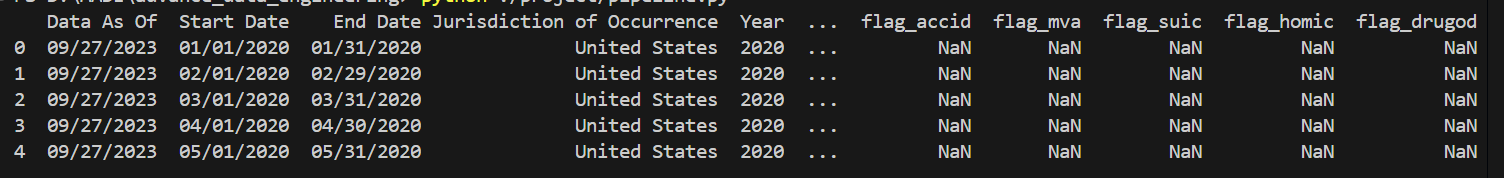
\includegraphics[width=0.9\textwidth]{images/dataset-1.png}
			\caption{First 5 rows of Monthly Provisional Counts of Deaths by Select Causes.}
			\label{fig:dataset1}
		\end{figure}
	\end{itemize}
	\begin{itemize}
		\item \textbf{U.S. Chronic Disease Indicators (CDI)} 
		
		The dataset is represented in tabular format were rows represent health indicators and columns is grouped by demographics (e.g., gender, race, geographic location). Key columns are Year, location, topic (is the indicator), questions and Datavalue. Some columns are empty but they are not needed for the analysis.
		\begin{figure}[ht!]
			\centering
			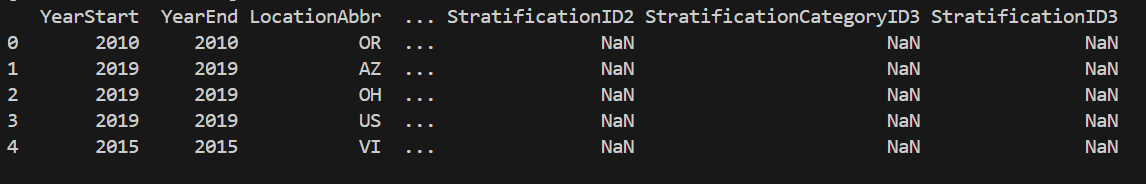
\includegraphics[width=0.9\textwidth]{images/dataset-2.png}
			\caption{First 5 rows of U.S. Chronic Disease Indicators (CDI).}
			\label{fig:dataset2}
		\end{figure}
		
	\end{itemize}

	\subsection{Licenses and Permissions}
	\begin{itemize}
	\item \textbf{Monthly Provisional Counts of Deaths by Select Causes (2020--2023)}
	
	The data is license under the \texttt{U.S. Government Work (Public Domain)}. The dataset is publicly available and produce by US Government. I can freely use this dataset to follow there restriction I will provide proper attribution to the U.S. government as the source of the data, While ensuring that I will not use any logo or anything that implies that it is endorse by the U.S. government. \cite{licenses2}
	\end{itemize}
	
	\begin{itemize}
	\item \textbf{U.S. Chronic Disease Indicators (CDI)} 
		
	This dataset is licensed under \texttt{Open Database License (ODbL)}. I am allow to free use this but need to provide proper attribution. I will adhere to this restriction by properly citing this dataset in my report and analysis. \cite{licenses1}
		
	\end{itemize}


	\subsection{Data Pipeline}
The data pipeline is developed using python. It contains three main modules: extract, transform, load. These modules contain respective functionalities.
 
 The pipeline begins by reading the metadata from a JSON file (\texttt{datasources.json}) to gather information about the data sources like URL, and columns to remove. The process starts by extracting the data from the URL using the \texttt{CsvExtractor} function, which retrieves the dataset in CSV format. Next, unnecessary columns are removed using the \texttt{DeleteColumns} function, based on the configuration provided in the metadata. If a filtering query is specified for the dataset, the \texttt{FilterRows} function is used to filter the data accordingly. Now, empty values in the dataset are filled using the \texttt{FillEmptyValues} function to ensure completeness. Finally, the transformed dataset is loaded into a SQLite database (\texttt{ChronicHealthTrends.db}) using the \texttt{LoadDfToSqlite} function, storing the data with the appropriate dataset name.
\begin{figure}[h]
	\centering
	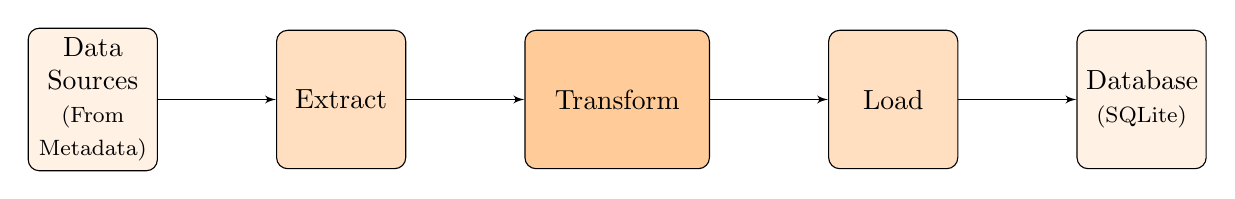
\begin{tikzpicture}[node distance=1.5cm and 1.5cm, auto]
		% Styles
		\tikzstyle{block} = [rectangle, draw, fill=orange!10,
		text width=4em, text centered, rounded corners, minimum height=5em]
		\tikzstyle{bigblock} = [rectangle, draw, fill=orange!25,
		text width=4em, text centered, rounded corners, minimum height=5em]
		\tikzstyle{biggerblock} = [rectangle, draw, fill=orange!40,
		text width=6em, text centered, rounded corners, minimum height=5em]
		\tikzstyle{line} = [draw, -latex', shorten >=0pt, shorten <=0pt]
		
		% Nodes
		\node [block] (sources) {Data Sources \footnotesize(From Metadata)};
		\node [bigblock, right=of sources] (extract) {Extract};
		\node [biggerblock, right=of extract] (transform) {Transform};
		\node [bigblock, right=of transform] (load) {Load};
		\node [block, right=of load] (database) {Database \footnotesize(SQLite)};
		
		% Connections
		\path [line] (sources) -- (extract);
		\path [line] (extract) -- (transform);
		\path [line] (transform) -- (load);
		\path [line] (load) -- (database);
	\end{tikzpicture}
	\caption{ETL Process Diagram}
	\label{fig:etl_process_diagram}
\end{figure}

	
\section{Results and Limitations}
Output result of the data pipeline is stored in SQLLite in table format as this is the most efficient and reliable way to store collective data. The pipeline can maintain the quality of data. The resultant datasets
\begin{itemize}
	\item fulfill the requirement that is needed to answer the questions.
	\item time domain is overlapping and fitting
	\item format is consistent
\end{itemize}

The datasets on chronic disease indicators and mortality statistics can be compared and analyzed to uncover correlations between chronic health conditions and mortality trends across various demographic and geographic segments. This enables a comprehensive understanding of the health factors contributing to death rates. However, a limitation arises with the granularity of chronic disease data, as it may not provide sufficient specificity to link certain health indicators directly to mortality causes.



\newpage
\bibliographystyle{plain}
\bibliography{references}

\end{document}
